\documentclass{whiteboard}
\begin{document}
\begin{frame}[plain,t]
\begin{tikzpicture}
\node[draw,opacity=0] at (0, 0) {x};
\node[draw,opacity=0] at (14, 8) {x};
 \node[circle, draw, very thick] (A) at (0, 4) { \bbtext{A} };
 \node[circle, draw, very thick] (B) at (6, 4) { \bbtext{B} };
 \node[circle, draw, very thick] (C) at (3, 1) { \bbtext{C} };
 \node[circle, draw, very thick] (D) at (3, 7) { \bbtext{D} };
 \draw[-latex,thick] (A) to node[above,pos=0.8] { \bbinfo{7} } (B);
 \draw[-latex,thick] (A) to node[right] { \bbinfo{1} } (C);
 \draw[-latex,thick] (C) to node[left,pos=0.7] { \bbinfo{2} } (D);
 \draw[-latex,thick] (D) to node[above] { \bbinfo{3} } (B);
\end{tikzpicture}
\end{frame}

\begin{frame}[plain,t]
\begin{tikzpicture}
\node[draw,opacity=0] at (0, 0) {x};
\node[draw,opacity=0] at (14, 8) {x};
 \node[circle, draw, very thick] (A) at (0, 4) { \bbtext{A} };
 \node[circle, draw, very thick] (B) at (6, 4) { \bbtext{B} };
 \node[circle, draw, very thick] (C) at (3, 1) { \bbtext{C} };
 \node[circle, draw, very thick] (D) at (3, 7) { \bbtext{D} };
 \draw[-latex,thick] (A) to node[above,pos=0.8] { \bbinfo{7} } (B);
 \draw[-latex,thick] (A) to node[right] { \bbinfo{1} } (C);
 \draw[-latex,thick] (C) to node[left,pos=0.7] { \bbinfo{2} } (D);
 \draw[-latex,thick] (D) to node[above] { \bbinfo{3} } (B);
 \draw[thick] (9, 5) grid (13, 6);
 \node[anchor=east] at (8.8, 5.5) { $\mathrm{dist}(u, \mbox{\bbtext{A}})$ };
 \node at (9.5, 6.3) { \bbtext{A} };
 \node at (10.5, 6.3) { \bbtext{B} };
 \node at (11.5, 6.3) { \bbtext{C} };
 \node at (12.5, 6.3) { \bbtext{D} };
 \node at (9.5, 5.5) { $0$ };
 \node at (10.5, 5.5) { $\infty$ };
 \node at (11.5, 5.5) { $\infty$ };
 \node at (12.5, 5.5) { $\infty$ };
\end{tikzpicture}
\end{frame}

\begin{frame}[plain,t]
\begin{tikzpicture}
\node[draw,opacity=0] at (0, 0) {x};
\node[draw,opacity=0] at (14, 8) {x};
 \node[circle, draw, very thick] (A) at (0, 4) { \bbtext{A} };
 \node[circle, draw, very thick] (B) at (6, 4) { \bbtext{B} };
 \node[circle, draw, very thick] (C) at (3, 1) { \bbtext{C} };
 \node[circle, draw, very thick] (D) at (3, 7) { \bbtext{D} };
 \draw[-latex,thick] (A) to node[above,pos=0.8] { \bbinfo{7} } (B);
 \draw[-latex,thick] (A) to node[right] { \bbinfo{1} } (C);
 \draw[-latex,thick] (C) to node[left,pos=0.7] { \bbinfo{2} } (D);
 \draw[-latex,thick] (D) to node[above] { \bbinfo{3} } (B);
 \draw[thick] (9, 5) grid (13, 6);
 \node[anchor=east] at (8.8, 5.5) { $\mathrm{dist}(u, \mbox{\bbtext{A}})$ };
 \node at (9.5, 6.3) { \bbtext{A} };
 \node at (10.5, 6.3) { \bbtext{B} };
 \node at (11.5, 6.3) { \bbtext{C} };
 \node at (12.5, 6.3) { \bbtext{D} };
 \node at (9.5, 5.5) { $0$ };
 \node at (10.5, 5.5) { $\infty$ };
 \node at (11.5, 5.5) { $\infty$ };
 \node at (12.5, 5.5) { $\infty$ };
 \draw[thick] (9, 2) grid (13, 3);
 \node[anchor=east] at (8.8, 2.5) { $\mathrm{pred}(u)$ };
 \node at (9.5, 3.3) { \bbtext{A} };
 \node at (10.5, 3.3) { \bbtext{B} };
 \node at (11.5, 3.3) { \bbtext{C} };
 \node at (12.5, 3.3) { \bbtext{D} };
 \node at (9.5, 2.5) { $\bbtext{A}$ };
 \node at (10.5, 2.5) { $\bbtext{-}$ };
 \node at (11.5, 2.5) { $\bbtext{-}$ };
 \node at (12.5, 2.5) { $\bbtext{-}$ };
\end{tikzpicture}
\end{frame}

\begin{frame}[plain,t]
\begin{tikzpicture}
\node[draw,opacity=0] at (0, 0) {x};
\node[draw,opacity=0] at (14, 8) {x};
 \node[circle, draw, very thick] (A) at (0, 4) { \bbtext{A} };
 \node[circle, draw, very thick] (B) at (6, 4) { \bbtext{B} };
 \node[circle, draw, very thick] (C) at (3, 1) { \bbtext{C} };
 \node[circle, draw, very thick] (D) at (3, 7) { \bbtext{D} };
 \draw[-latex,thick] (A) to node[right] { \bbinfo{1} } (C);
 \draw[-latex,thick] (C) to node[left,pos=0.7] { \bbinfo{2} } (D);
 \draw[-latex,thick] (D) to node[above] { \bbinfo{3} } (B);
 \draw[thick] (9, 5) grid (13, 6);
 \node[anchor=east] at (8.8, 5.5) { $\mathrm{dist}(u, \mbox{\bbtext{A}})$ };
 \node at (9.5, 6.3) { \bbtext{A} };
 \node at (10.5, 6.3) { \bbtext{B} };
 \node at (11.5, 6.3) { \bbtext{C} };
 \node at (12.5, 6.3) { \bbtext{D} };
 \node at (9.5, 5.5) { $0$ };
 \node at (11.5, 5.5) { $\infty$ };
 \node at (12.5, 5.5) { $\infty$ };
 \draw[thick] (9, 2) grid (13, 3);
 \node[anchor=east] at (8.8, 2.5) { $\mathrm{pred}(u)$ };
 \node at (9.5, 3.3) { \bbtext{A} };
 \node at (10.5, 3.3) { \bbtext{B} };
 \node at (11.5, 3.3) { \bbtext{C} };
 \node at (12.5, 3.3) { \bbtext{D} };
 \node at (9.5, 2.5) { $\bbtext{A}$ };
 \node at (11.5, 2.5) { $\bbtext{-}$ };
 \node at (12.5, 2.5) { $\bbtext{-}$ };
 \draw[-latex,very thick,color=BBCyan] (A) to node[above,pos=0.8] { \bbinfo{7} } (B);
 \node at (10.5, 5.5) { $\mathbf{7}$ };
 \node at (10.5, 2.5) { $\bbupdate{A}$ };
\end{tikzpicture}
\end{frame}

\begin{frame}[plain,t]
\begin{tikzpicture}
\node[draw,opacity=0] at (0, 0) {x};
\node[draw,opacity=0] at (14, 8) {x};
 \node[circle, draw, very thick] (A) at (0, 4) { \bbtext{A} };
 \node[circle, draw, very thick] (B) at (6, 4) { \bbtext{B} };
 \node[circle, draw, very thick] (C) at (3, 1) { \bbtext{C} };
 \node[circle, draw, very thick] (D) at (3, 7) { \bbtext{D} };
 \draw[-latex,thick] (C) to node[left,pos=0.7] { \bbinfo{2} } (D);
 \draw[-latex,thick] (D) to node[above] { \bbinfo{3} } (B);
 \draw[thick] (9, 5) grid (13, 6);
 \node[anchor=east] at (8.8, 5.5) { $\mathrm{dist}(u, \mbox{\bbtext{A}})$ };
 \node at (9.5, 6.3) { \bbtext{A} };
 \node at (10.5, 6.3) { \bbtext{B} };
 \node at (11.5, 6.3) { \bbtext{C} };
 \node at (12.5, 6.3) { \bbtext{D} };
 \node at (9.5, 5.5) { $0$ };
 \node at (12.5, 5.5) { $\infty$ };
 \draw[thick] (9, 2) grid (13, 3);
 \node[anchor=east] at (8.8, 2.5) { $\mathrm{pred}(u)$ };
 \node at (9.5, 3.3) { \bbtext{A} };
 \node at (10.5, 3.3) { \bbtext{B} };
 \node at (11.5, 3.3) { \bbtext{C} };
 \node at (12.5, 3.3) { \bbtext{D} };
 \node at (9.5, 2.5) { $\bbtext{A}$ };
 \node at (12.5, 2.5) { $\bbtext{-}$ };
 \draw[-latex,thick] (A) to node[above,pos=0.8] { \bbinfo{7} } (B);
 \node at (10.5, 5.5) { $7$ };
 \node at (10.5, 2.5) { $\bbtext{A}$ };
 \draw[-latex,very thick,color=BBCyan] (A) to node[right] { \bbinfo{1} } (C);
 \node at (11.5, 5.5) { $\mathbf{1}$ };
 \node at (11.5, 2.5) { $\bbupdate{A}$ };
\end{tikzpicture}
\end{frame}

\begin{frame}[plain,t]
\begin{tikzpicture}
\node[draw,opacity=0] at (0, 0) {x};
\node[draw,opacity=0] at (14, 8) {x};
 \node[circle, draw, very thick] (A) at (0, 4) { \bbtext{A} };
 \node[circle, draw, very thick] (B) at (6, 4) { \bbtext{B} };
 \node[circle, draw, very thick] (C) at (3, 1) { \bbtext{C} };
 \node[circle, draw, very thick] (D) at (3, 7) { \bbtext{D} };
 \draw[-latex,thick] (D) to node[above] { \bbinfo{3} } (B);
 \draw[thick] (9, 5) grid (13, 6);
 \node[anchor=east] at (8.8, 5.5) { $\mathrm{dist}(u, \mbox{\bbtext{A}})$ };
 \node at (9.5, 6.3) { \bbtext{A} };
 \node at (10.5, 6.3) { \bbtext{B} };
 \node at (11.5, 6.3) { \bbtext{C} };
 \node at (12.5, 6.3) { \bbtext{D} };
 \node at (9.5, 5.5) { $0$ };
 \draw[thick] (9, 2) grid (13, 3);
 \node[anchor=east] at (8.8, 2.5) { $\mathrm{pred}(u)$ };
 \node at (9.5, 3.3) { \bbtext{A} };
 \node at (10.5, 3.3) { \bbtext{B} };
 \node at (11.5, 3.3) { \bbtext{C} };
 \node at (12.5, 3.3) { \bbtext{D} };
 \node at (9.5, 2.5) { $\bbtext{A}$ };
 \draw[-latex,thick] (A) to node[above,pos=0.8] { \bbinfo{7} } (B);
 \node at (10.5, 5.5) { $7$ };
 \node at (10.5, 2.5) { $\bbtext{A}$ };
 \node at (11.5, 5.5) { ${1}$ };
 \node at (11.5, 2.5) { $\bbtext{A}$ };
 \draw[-latex,thick] (A) to node[right] { \bbinfo{1} } (C);
 \draw[-latex,very thick,color=BBCyan] (C) to node[left,pos=0.7] { \bbinfo{2} } (D);
 \node at (12.5, 2.5) { $\bbupdate{C}$ };
 \node at (12.5, 5.5) { $\mathbf{3}$ };
\end{tikzpicture}
\end{frame}

\begin{frame}[plain,t]
\begin{tikzpicture}
\node[draw,opacity=0] at (0, 0) {x};
\node[draw,opacity=0] at (14, 8) {x};
 \node[circle, draw, very thick] (A) at (0, 4) { \bbtext{A} };
 \node[circle, draw, very thick] (B) at (6, 4) { \bbtext{B} };
 \node[circle, draw, very thick] (C) at (3, 1) { \bbtext{C} };
 \node[circle, draw, very thick] (D) at (3, 7) { \bbtext{D} };
 \draw[thick] (9, 5) grid (13, 6);
 \node[anchor=east] at (8.8, 5.5) { $\mathrm{dist}(u, \mbox{\bbtext{A}})$ };
 \node at (9.5, 6.3) { \bbtext{A} };
 \node at (10.5, 6.3) { \bbtext{B} };
 \node at (11.5, 6.3) { \bbtext{C} };
 \node at (12.5, 6.3) { \bbtext{D} };
 \node at (9.5, 5.5) { $0$ };
 \draw[thick] (9, 2) grid (13, 3);
 \node[anchor=east] at (8.8, 2.5) { $\mathrm{pred}(u)$ };
 \node at (9.5, 3.3) { \bbtext{A} };
 \node at (10.5, 3.3) { \bbtext{B} };
 \node at (11.5, 3.3) { \bbtext{C} };
 \node at (12.5, 3.3) { \bbtext{D} };
 \node at (9.5, 2.5) { $\bbtext{A}$ };
 \draw[-latex,thick] (A) to node[above,pos=0.8] { \bbinfo{7} } (B);
 \node at (11.5, 5.5) { ${1}$ };
 \node at (11.5, 2.5) { $\bbtext{A}$ };
 \draw[-latex,thick] (A) to node[right] { \bbinfo{1} } (C);
 \node at (12.5, 2.5) { $\bbtext{C}$ };
 \node at (12.5, 5.5) { ${3}$ };
 \draw[-latex,thick] (C) to node[left,pos=0.7] { \bbinfo{2} } (D);
 \draw[-latex,very thick,color=BBCyan] (D) to node[above] { \bbinfo{3} } (B);
 \node at (10.5, 5.5) { $\mathbf{6}$ };
 \node at (10.5, 2.5) { $\bbupdate{D}$ };
\end{tikzpicture}
\end{frame}

\begin{frame}[plain,t]
\begin{tikzpicture}
\node[draw,opacity=0] at (0, 0) {x};
\node[draw,opacity=0] at (14, 8) {x};
 \node[circle, draw, very thick] (A) at (0, 4) { \bbtext{A} };
 \node[circle, draw, very thick] (B) at (6, 4) { \bbtext{B} };
 \node[circle, draw, very thick] (C) at (3, 1) { \bbtext{C} };
 \node[circle, draw, very thick] (D) at (3, 7) { \bbtext{D} };
 \draw[thick] (9, 5) grid (13, 6);
 \node[anchor=east] at (8.8, 5.5) { $\mathrm{dist}(u, \mbox{\bbtext{A}})$ };
 \node at (9.5, 6.3) { \bbtext{A} };
 \node at (10.5, 6.3) { \bbtext{B} };
 \node at (11.5, 6.3) { \bbtext{C} };
 \node at (12.5, 6.3) { \bbtext{D} };
 \node at (9.5, 5.5) { $0$ };
 \draw[thick] (9, 2) grid (13, 3);
 \node[anchor=east] at (8.8, 2.5) { $\mathrm{pred}(u)$ };
 \node at (9.5, 3.3) { \bbtext{A} };
 \node at (10.5, 3.3) { \bbtext{B} };
 \node at (11.5, 3.3) { \bbtext{C} };
 \node at (12.5, 3.3) { \bbtext{D} };
 \node at (9.5, 2.5) { $\bbtext{A}$ };
 \draw[-latex,thick] (A) to node[above,pos=0.8] { \bbinfo{7} } (B);
 \node at (11.5, 5.5) { ${1}$ };
 \node at (11.5, 2.5) { $\bbtext{A}$ };
 \draw[-latex,thick] (A) to node[right] { \bbinfo{1} } (C);
 \node at (12.5, 2.5) { $\bbtext{C}$ };
 \node at (12.5, 5.5) { ${3}$ };
 \draw[-latex,thick] (C) to node[left,pos=0.7] { \bbinfo{2} } (D);
 \node at (10.5, 2.5) { $\bbtext{D}$ };
 \draw[-latex,thick] (D) to node[above] { \bbinfo{3} } (B);
 \node at (10.5, 5.5) { ${6}$ };
 \draw[latex-,thick,color=BBViolet] (B) to [bend right] node[above right] { \tiny $(\mathrm{prev}(\mbox{\bbtext{B}}), \mbox{\bbtext{B}})$ } (D);
\end{tikzpicture}
\end{frame}

\begin{frame}[plain,t]
\begin{tikzpicture}
\node[draw,opacity=0] at (0, 0) {x};
\node[draw,opacity=0] at (14, 8) {x};
 \node[circle, draw, very thick] (A) at (0, 4) { \bbtext{A} };
 \node[circle, draw, very thick] (B) at (6, 4) { \bbtext{B} };
 \node[circle, draw, very thick] (C) at (3, 1) { \bbtext{C} };
 \node[circle, draw, very thick] (D) at (3, 7) { \bbtext{D} };
 \draw[thick] (9, 5) grid (13, 6);
 \node[anchor=east] at (8.8, 5.5) { $\mathrm{dist}(u, \mbox{\bbtext{A}})$ };
 \node at (9.5, 6.3) { \bbtext{A} };
 \node at (10.5, 6.3) { \bbtext{B} };
 \node at (11.5, 6.3) { \bbtext{C} };
 \node at (12.5, 6.3) { \bbtext{D} };
 \node at (9.5, 5.5) { $0$ };
 \draw[thick] (9, 2) grid (13, 3);
 \node[anchor=east] at (8.8, 2.5) { $\mathrm{pred}(u)$ };
 \node at (9.5, 3.3) { \bbtext{A} };
 \node at (10.5, 3.3) { \bbtext{B} };
 \node at (11.5, 3.3) { \bbtext{C} };
 \node at (12.5, 3.3) { \bbtext{D} };
 \node at (9.5, 2.5) { $\bbtext{A}$ };
 \draw[-latex,thick] (A) to node[above,pos=0.8] { \bbinfo{7} } (B);
 \node at (11.5, 5.5) { ${1}$ };
 \node at (11.5, 2.5) { $\bbtext{A}$ };
 \draw[-latex,thick] (A) to node[right] { \bbinfo{1} } (C);
 \node at (12.5, 2.5) { $\bbtext{C}$ };
 \node at (12.5, 5.5) { ${3}$ };
 \draw[-latex,thick] (C) to node[left,pos=0.7] { \bbinfo{2} } (D);
 \node at (10.5, 2.5) { $\bbtext{D}$ };
 \draw[-latex,thick] (D) to node[above] { \bbinfo{3} } (B);
 \node at (10.5, 5.5) { ${6}$ };
 \draw[latex-,thick,color=BBViolet] (B) to [bend right] node[above right] { \tiny $(\mathrm{prev}(\mbox{\bbtext{B}}), \mbox{\bbtext{B}})$ } (D);
 \draw[-latex,thick,color=BBViolet] (C) to [bend right] node[right, pos=0.3] { \tiny $(\mathrm{prev}(\mbox{\bbtext{D}}), \mbox{\bbtext{D}})$ } (D);
\end{tikzpicture}
\end{frame}

\begin{frame}[plain,t]
\begin{tikzpicture}
\node[draw,opacity=0] at (0, 0) {x};
\node[draw,opacity=0] at (14, 8) {x};
 \node[circle, draw, very thick] (A) at (0, 4) { \bbtext{A} };
 \node[circle, draw, very thick] (B) at (6, 4) { \bbtext{B} };
 \node[circle, draw, very thick] (C) at (3, 1) { \bbtext{C} };
 \node[circle, draw, very thick] (D) at (3, 7) { \bbtext{D} };
 \draw[thick] (9, 5) grid (13, 6);
 \node[anchor=east] at (8.8, 5.5) { $\mathrm{dist}(u, \mbox{\bbtext{A}})$ };
 \node at (9.5, 6.3) { \bbtext{A} };
 \node at (10.5, 6.3) { \bbtext{B} };
 \node at (11.5, 6.3) { \bbtext{C} };
 \node at (12.5, 6.3) { \bbtext{D} };
 \node at (9.5, 5.5) { $0$ };
 \draw[thick] (9, 2) grid (13, 3);
 \node[anchor=east] at (8.8, 2.5) { $\mathrm{pred}(u)$ };
 \node at (9.5, 3.3) { \bbtext{A} };
 \node at (10.5, 3.3) { \bbtext{B} };
 \node at (11.5, 3.3) { \bbtext{C} };
 \node at (12.5, 3.3) { \bbtext{D} };
 \node at (9.5, 2.5) { $\bbtext{A}$ };
 \draw[-latex,thick] (A) to node[above,pos=0.8] { \bbinfo{7} } (B);
 \node at (11.5, 5.5) { ${1}$ };
 \node at (11.5, 2.5) { $\bbtext{A}$ };
 \draw[-latex,thick] (A) to node[right] { \bbinfo{1} } (C);
 \node at (12.5, 2.5) { $\bbtext{C}$ };
 \node at (12.5, 5.5) { ${3}$ };
 \draw[-latex,thick] (C) to node[left,pos=0.7] { \bbinfo{2} } (D);
 \node at (10.5, 2.5) { $\bbtext{D}$ };
 \draw[-latex,thick] (D) to node[above] { \bbinfo{3} } (B);
 \node at (10.5, 5.5) { ${6}$ };
 \draw[latex-,thick,color=BBViolet] (B) to [bend right] node[above right] { \tiny $(\mathrm{prev}(\mbox{\bbtext{B}}), \mbox{\bbtext{B}})$ } (D);
 \draw[-latex,thick,color=BBViolet] (C) to [bend right] node[right, pos=0.3] { \tiny $(\mathrm{prev}(\mbox{\bbtext{D}}), \mbox{\bbtext{D}})$ } (D);
 \draw[-latex,thick,color=BBViolet] (A) to [bend right] node[below left, pos=0.3] { \tiny $(\mathrm{prev}(\mbox{\bbtext{C}}), \mbox{\bbtext{C}})$ } (C);
\end{tikzpicture}
\end{frame}

\begin{frame}[plain,t]
 \begin{center}\inputsnippet{cpp}{9}{25}{codes/bellman-ford-path.cpp}\end{center}
\end{frame}

\begin{frame}[plain,t]
 \begin{center}\inputsnippet{cpp}{27}{40}{codes/bellman-ford-path.cpp}\end{center}
\end{frame}

\begin{frame}[plain,t]
\begin{tikzpicture}
\node[draw,opacity=0] at (0, 0) {x};
\node[draw,opacity=0] at (14, 8) {x};
 \node[anchor=west] at (0, 7) { \Large \bbbold{Caminhos mínimos e ciclos} };
\end{tikzpicture}
\end{frame}

\begin{frame}[plain,t]
\begin{tikzpicture}
\node[draw,opacity=0] at (0, 0) {x};
\node[draw,opacity=0] at (14, 8) {x};
 \node[anchor=west] at (0, 7) { \Large \bbbold{Caminhos mínimos e ciclos} };
 \node[anchor=west] at (1, 6) { \bbtext{Seja} };
 \node[anchor=west] at (2, 5) { $p = \{ (a, u_1), (u_1, u_2), \ldots, (v, u_r), \dots, (u_s, v), \ldots, (u_t, b) \}$ };
 \node[anchor=west] at (0.5, 4) { \bbtext{um caminho de $a$ a $b$ e $\omega(c)$ o custo do ciclo $c = \{ (v, u_r), \ldots, (u_s, v) \}$, isto é } };
 \node[anchor=west] at (5, 3) { $\displaystyle{\omega(c) = \sum_{e\in c} w(e)}$ };
\end{tikzpicture}
\end{frame}

\begin{frame}[plain,t]
\begin{tikzpicture}
\node[draw,opacity=0] at (0, 0) {x};
\node[draw,opacity=0] at (14, 8) {x};
 \node[anchor=west] at (0, 7) { \Large \bbbold{Caminhos mínimos e ciclos} };
 \node[anchor=west] at (1, 6) { \bbtext{Seja} };
 \node[anchor=west] at (2, 5) { $p = \{ (a, u_1), (u_1, u_2), \ldots, (v, u_r), \dots, (u_s, v), \ldots, (u_t, b) \}$ };
 \node[anchor=west] at (0.5, 4) { \bbtext{um caminho de $a$ a $b$ e $\omega(c)$ o custo do ciclo $c = \{ (v, u_r), \ldots, (u_s, v) \}$, isto é } };
 \node[anchor=west] at (5, 3) { $\displaystyle{\omega(c) = \sum_{e\in c} w(e)}$ };
 \draw[-latex,color=BBViolet] (7.3, 2.8) to (7.3, 2.6) to (10, 2.6);
 \node[anchor=west] at (10, 2.6) { \footnotesize \bbcomment{custo da aresta $e$} };
\end{tikzpicture}
\end{frame}

\begin{frame}[plain,t]
\begin{tikzpicture}
\node[draw,opacity=0] at (0, 0) {x};
\node[draw,opacity=0] at (14, 8) {x};
 \node[anchor=west] at (0, 7) { \Large \bbbold{Caminhos mínimos e ciclos} };
 \node[anchor=west] at (1, 6) { \bbtext{Seja} };
 \node[anchor=west] at (2, 5) { $p = \{ (a, u_1), (u_1, u_2), \ldots, (v, u_r), \dots, (u_s, v), \ldots, (u_t, b) \}$ };
 \node[anchor=west] at (0.5, 4) { \bbtext{um caminho de $a$ a $b$ e $\omega(c)$ o custo do ciclo $c = \{ (v, u_r), \ldots, (u_s, v) \}$, isto é } };
 \node[anchor=west] at (5, 3) { $\displaystyle{\omega(c) = \sum_{e\in c} w(e)}$ };
 \draw[-latex,color=BBViolet] (7.3, 2.8) to (7.3, 2.6) to (10, 2.6);
 \node[anchor=west] at (10, 2.6) { \footnotesize \bbcomment{custo da aresta $e$} };
 \node[anchor=west] at (0.5, 2) { \bbtext{Se $p$ é caminho mínimo de $a$ a $b$ então $\omega(c) = 0$.} };
\end{tikzpicture}
\end{frame}

\begin{frame}[plain,t]
\begin{tikzpicture}
\node[draw,opacity=0] at (0, 0) {x};
\node[draw,opacity=0] at (14, 8) {x};
 \node[anchor=west] at (0, 6.5) { \Large \bbbold{Caminhos mínimos e ciclos positivos} };
\end{tikzpicture}
\end{frame}

\begin{frame}[plain,t]
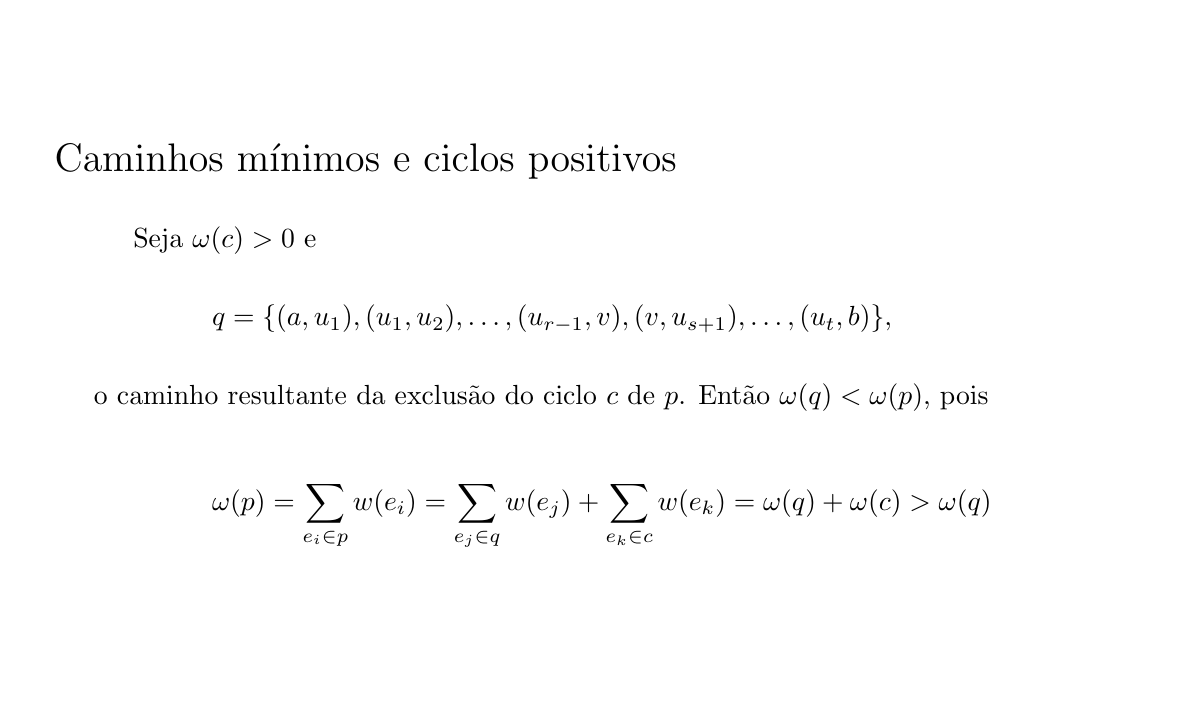
\begin{tikzpicture}
\node[draw,opacity=0] at (0, 0) {x};
\node[draw,opacity=0] at (14, 8) {x};
 \node[anchor=west] at (0, 6.5) { \Large \bbbold{Caminhos mínimos e ciclos positivos} };
 \node[anchor=west] at (1, 5.5) { \bbtext{Seja $\omega(c) > 0$ e } };
 \node[anchor=west] at (2, 4.5) { $q = \{ (a, u_1), (u_1, u_2), \ldots, (u_{r - 1}, v), (v, u_{s + 1}), \ldots, (u_t, b) \},$ };
 \node[anchor=west] at (0.5, 3.5) { \bbtext{o caminho resultante da exclusão do ciclo $c$ de $p$. Então $\omega(q) < \omega(p)$, pois} };
 \node[anchor=west] at (2, 2) { $ \omega(p) = \displaystyle{\sum_{e_i\in p} w(e_i) = \sum_{e_j\in q} w(e_j) + \sum_{e_k\in c} w(e_k) = \omega(q) + \omega(c) > \omega(q)} $ };
\end{tikzpicture}
\end{frame}

\begin{frame}[plain,t]
\begin{tikzpicture}
\node[draw,opacity=0] at (0, 0) {x};
\node[draw,opacity=0] at (14, 8) {x};
 \node[circle, draw, very thick] (A) at (0.5, 7) { \bbtext{A} };
 \node[circle, draw, very thick] (B) at (6.5, 7) { \bbtext{B} };
 \node[circle, draw, very thick] (C) at (12.5, 7) { \bbtext{C} };
 \node[circle, draw, very thick] (D) at (9.5, 5) { \bbtext{D} };
 \node[circle, draw, very thick] (E) at (6.5, 3) { \bbtext{E} };
 \node[circle, draw, very thick] (F) at (3.5, 5) { \bbtext{F} };
 \draw[thick] (A) to node[below] { \bbinfo{1} } (B);
 \draw[thick] (B) to node[below] { \bbinfo{2} } (C);
 \draw[thick] (B) to node[below] { \bbinfo{3} } (D);
 \draw[thick] (D) to node[below] { \bbinfo{4} } (E);
 \draw[thick] (E) to node[below] { \bbinfo{5} } (F);
 \draw[thick] (F) to node[below] { \bbinfo{-6} } (B);
\end{tikzpicture}
\end{frame}

\begin{frame}[plain,t]
\begin{tikzpicture}
\node[draw,opacity=0] at (0, 0) {x};
\node[draw,opacity=0] at (14, 8) {x};
 \node[circle, draw, very thick] (A) at (0.5, 7) { \bbtext{A} };
 \node[circle, draw, very thick] (B) at (6.5, 7) { \bbtext{B} };
 \node[circle, draw, very thick] (C) at (12.5, 7) { \bbtext{C} };
 \node[circle, draw, very thick] (D) at (9.5, 5) { \bbtext{D} };
 \node[circle, draw, very thick] (E) at (6.5, 3) { \bbtext{E} };
 \node[circle, draw, very thick] (F) at (3.5, 5) { \bbtext{F} };
 \draw[thick] (A) to node[below] { \bbinfo{1} } (B);
 \draw[thick] (B) to node[below] { \bbinfo{2} } (C);
 \draw[thick] (B) to node[below] { \bbinfo{3} } (D);
 \draw[thick] (D) to node[below] { \bbinfo{4} } (E);
 \draw[thick] (E) to node[below] { \bbinfo{5} } (F);
 \draw[thick] (F) to node[below] { \bbinfo{-6} } (B);
 \draw[-latex,color=BBCyan] (1, 2) to (2, 2);
 \node[anchor=west] at (2, 2) { $p$ };
\end{tikzpicture}
\end{frame}

\begin{frame}[plain,t]
\begin{tikzpicture}
\node[draw,opacity=0] at (0, 0) {x};
\node[draw,opacity=0] at (14, 8) {x};
 \node[circle, draw, very thick] (A) at (0.5, 7) { \bbtext{A} };
 \node[circle, draw, very thick] (B) at (6.5, 7) { \bbtext{B} };
 \node[circle, draw, very thick] (C) at (12.5, 7) { \bbtext{C} };
 \node[circle, draw, very thick] (D) at (9.5, 5) { \bbtext{D} };
 \node[circle, draw, very thick] (E) at (6.5, 3) { \bbtext{E} };
 \node[circle, draw, very thick] (F) at (3.5, 5) { \bbtext{F} };
 \draw[thick] (B) to node[below] { \bbinfo{2} } (C);
 \draw[thick] (B) to node[below] { \bbinfo{3} } (D);
 \draw[thick] (D) to node[below] { \bbinfo{4} } (E);
 \draw[thick] (E) to node[below] { \bbinfo{5} } (F);
 \draw[thick] (F) to node[below] { \bbinfo{-6} } (B);
 \draw[-latex,color=BBCyan] (1, 2) to (2, 2);
 \node[anchor=west] at (2, 2) { $p$ };
 \draw[-latex,very thick,color=BBCyan] (A) to node[below] { \bbinfo{1} } (B);
\end{tikzpicture}
\end{frame}

\begin{frame}[plain,t]
\begin{tikzpicture}
\node[draw,opacity=0] at (0, 0) {x};
\node[draw,opacity=0] at (14, 8) {x};
 \node[circle, draw, very thick] (A) at (0.5, 7) { \bbtext{A} };
 \node[circle, draw, very thick] (B) at (6.5, 7) { \bbtext{B} };
 \node[circle, draw, very thick] (C) at (12.5, 7) { \bbtext{C} };
 \node[circle, draw, very thick] (D) at (9.5, 5) { \bbtext{D} };
 \node[circle, draw, very thick] (E) at (6.5, 3) { \bbtext{E} };
 \node[circle, draw, very thick] (F) at (3.5, 5) { \bbtext{F} };
 \draw[thick] (B) to node[below] { \bbinfo{2} } (C);
 \draw[thick] (D) to node[below] { \bbinfo{4} } (E);
 \draw[thick] (E) to node[below] { \bbinfo{5} } (F);
 \draw[thick] (F) to node[below] { \bbinfo{-6} } (B);
 \draw[-latex,color=BBCyan] (1, 2) to (2, 2);
 \node[anchor=west] at (2, 2) { $p$ };
 \draw[-latex,very thick,color=BBCyan] (A) to node[below] { \bbinfo{1} } (B);
 \draw[-latex,very thick,color=BBCyan] (B) to node[below] { \bbinfo{3} } (D);
\end{tikzpicture}
\end{frame}

\begin{frame}[plain,t]
\begin{tikzpicture}
\node[draw,opacity=0] at (0, 0) {x};
\node[draw,opacity=0] at (14, 8) {x};
 \node[circle, draw, very thick] (A) at (0.5, 7) { \bbtext{A} };
 \node[circle, draw, very thick] (B) at (6.5, 7) { \bbtext{B} };
 \node[circle, draw, very thick] (C) at (12.5, 7) { \bbtext{C} };
 \node[circle, draw, very thick] (D) at (9.5, 5) { \bbtext{D} };
 \node[circle, draw, very thick] (E) at (6.5, 3) { \bbtext{E} };
 \node[circle, draw, very thick] (F) at (3.5, 5) { \bbtext{F} };
 \draw[thick] (B) to node[below] { \bbinfo{2} } (C);
 \draw[thick] (E) to node[below] { \bbinfo{5} } (F);
 \draw[thick] (F) to node[below] { \bbinfo{-6} } (B);
 \draw[-latex,color=BBCyan] (1, 2) to (2, 2);
 \node[anchor=west] at (2, 2) { $p$ };
 \draw[-latex,very thick,color=BBCyan] (A) to node[below] { \bbinfo{1} } (B);
 \draw[-latex,very thick,color=BBCyan] (B) to node[below] { \bbinfo{3} } (D);
 \draw[-latex,very thick,color=BBCyan] (D) to node[below] { \bbinfo{4} } (E);
\end{tikzpicture}
\end{frame}

\begin{frame}[plain,t]
\begin{tikzpicture}
\node[draw,opacity=0] at (0, 0) {x};
\node[draw,opacity=0] at (14, 8) {x};
 \node[circle, draw, very thick] (A) at (0.5, 7) { \bbtext{A} };
 \node[circle, draw, very thick] (B) at (6.5, 7) { \bbtext{B} };
 \node[circle, draw, very thick] (C) at (12.5, 7) { \bbtext{C} };
 \node[circle, draw, very thick] (D) at (9.5, 5) { \bbtext{D} };
 \node[circle, draw, very thick] (E) at (6.5, 3) { \bbtext{E} };
 \node[circle, draw, very thick] (F) at (3.5, 5) { \bbtext{F} };
 \draw[thick] (B) to node[below] { \bbinfo{2} } (C);
 \draw[thick] (F) to node[below] { \bbinfo{-6} } (B);
 \draw[-latex,color=BBCyan] (1, 2) to (2, 2);
 \node[anchor=west] at (2, 2) { $p$ };
 \draw[-latex,very thick,color=BBCyan] (A) to node[below] { \bbinfo{1} } (B);
 \draw[-latex,very thick,color=BBCyan] (B) to node[below] { \bbinfo{3} } (D);
 \draw[-latex,very thick,color=BBCyan] (D) to node[below] { \bbinfo{4} } (E);
 \draw[-latex,very thick,color=BBCyan] (E) to node[below] { \bbinfo{5} } (F);
\end{tikzpicture}
\end{frame}

\begin{frame}[plain,t]
\begin{tikzpicture}
\node[draw,opacity=0] at (0, 0) {x};
\node[draw,opacity=0] at (14, 8) {x};
 \node[circle, draw, very thick] (A) at (0.5, 7) { \bbtext{A} };
 \node[circle, draw, very thick] (B) at (6.5, 7) { \bbtext{B} };
 \node[circle, draw, very thick] (C) at (12.5, 7) { \bbtext{C} };
 \node[circle, draw, very thick] (D) at (9.5, 5) { \bbtext{D} };
 \node[circle, draw, very thick] (E) at (6.5, 3) { \bbtext{E} };
 \node[circle, draw, very thick] (F) at (3.5, 5) { \bbtext{F} };
 \draw[thick] (B) to node[below] { \bbinfo{2} } (C);
 \draw[-latex,color=BBCyan] (1, 2) to (2, 2);
 \node[anchor=west] at (2, 2) { $p$ };
 \draw[-latex,very thick,color=BBCyan] (A) to node[below] { \bbinfo{1} } (B);
 \draw[-latex,very thick,color=BBCyan] (B) to node[below] { \bbinfo{3} } (D);
 \draw[-latex,very thick,color=BBCyan] (D) to node[below] { \bbinfo{4} } (E);
 \draw[-latex,very thick,color=BBCyan] (E) to node[below] { \bbinfo{5} } (F);
 \draw[-latex,very thick,color=BBCyan] (F) to node[below] { \bbinfo{-6} } (B);
\end{tikzpicture}
\end{frame}

\begin{frame}[plain,t]
\begin{tikzpicture}
\node[draw,opacity=0] at (0, 0) {x};
\node[draw,opacity=0] at (14, 8) {x};
 \node[circle, draw, very thick] (A) at (0.5, 7) { \bbtext{A} };
 \node[circle, draw, very thick] (B) at (6.5, 7) { \bbtext{B} };
 \node[circle, draw, very thick] (C) at (12.5, 7) { \bbtext{C} };
 \node[circle, draw, very thick] (D) at (9.5, 5) { \bbtext{D} };
 \node[circle, draw, very thick] (E) at (6.5, 3) { \bbtext{E} };
 \node[circle, draw, very thick] (F) at (3.5, 5) { \bbtext{F} };
 \draw[-latex,color=BBCyan] (1, 2) to (2, 2);
 \node[anchor=west] at (2, 2) { $p$ };
 \draw[-latex,very thick,color=BBCyan] (A) to node[below] { \bbinfo{1} } (B);
 \draw[-latex,very thick,color=BBCyan] (B) to node[below] { \bbinfo{3} } (D);
 \draw[-latex,very thick,color=BBCyan] (D) to node[below] { \bbinfo{4} } (E);
 \draw[-latex,very thick,color=BBCyan] (E) to node[below] { \bbinfo{5} } (F);
 \draw[-latex,very thick,color=BBCyan] (F) to node[below] { \bbinfo{-6} } (B);
 \draw[-latex,very thick,color=BBCyan] (B) to node[below] { \bbinfo{2} } (C);
\end{tikzpicture}
\end{frame}

\begin{frame}[plain,t]
\begin{tikzpicture}
\node[draw,opacity=0] at (0, 0) {x};
\node[draw,opacity=0] at (14, 8) {x};
 \node[circle, draw, very thick] (A) at (0.5, 7) { \bbtext{A} };
 \node[circle, draw, very thick] (B) at (6.5, 7) { \bbtext{B} };
 \node[circle, draw, very thick] (C) at (12.5, 7) { \bbtext{C} };
 \node[circle, draw, very thick] (D) at (9.5, 5) { \bbtext{D} };
 \node[circle, draw, very thick] (E) at (6.5, 3) { \bbtext{E} };
 \node[circle, draw, very thick] (F) at (3.5, 5) { \bbtext{F} };
 \draw[-latex,color=BBCyan] (1, 2) to (2, 2);
 \node[anchor=west] at (2, 2) { $p$ };
 \draw[-latex,very thick,color=BBCyan] (A) to node[below] { \bbinfo{1} } (B);
 \draw[-latex,very thick,color=BBCyan] (B) to node[below] { \bbinfo{3} } (D);
 \draw[-latex,very thick,color=BBCyan] (D) to node[below] { \bbinfo{4} } (E);
 \draw[-latex,very thick,color=BBCyan] (E) to node[below] { \bbinfo{5} } (F);
 \draw[-latex,very thick,color=BBCyan] (F) to node[below] { \bbinfo{-6} } (B);
 \draw[-latex,very thick,color=BBCyan] (B) to node[below] { \bbinfo{2} } (C);
 \node[anchor=west] at (3, 2) { $\omega(p) = 9$ };
\end{tikzpicture}
\end{frame}

\begin{frame}[plain,t]
\begin{tikzpicture}
\node[draw,opacity=0] at (0, 0) {x};
\node[draw,opacity=0] at (14, 8) {x};
 \node[circle, draw, very thick] (A) at (0.5, 7) { \bbtext{A} };
 \node[circle, draw, very thick] (B) at (6.5, 7) { \bbtext{B} };
 \node[circle, draw, very thick] (C) at (12.5, 7) { \bbtext{C} };
 \node[circle, draw, very thick] (D) at (9.5, 5) { \bbtext{D} };
 \node[circle, draw, very thick] (E) at (6.5, 3) { \bbtext{E} };
 \node[circle, draw, very thick] (F) at (3.5, 5) { \bbtext{F} };
 \draw[-latex,color=BBCyan] (1, 2) to (2, 2);
 \node[anchor=west] at (2, 2) { $p$ };
 \draw[-latex,very thick,color=BBCyan] (A) to node[below] { \bbinfo{1} } (B);
 \draw[-latex,very thick,color=BBCyan] (B) to node[below] { \bbinfo{3} } (D);
 \draw[-latex,very thick,color=BBCyan] (D) to node[below] { \bbinfo{4} } (E);
 \draw[-latex,very thick,color=BBCyan] (E) to node[below] { \bbinfo{5} } (F);
 \draw[-latex,very thick,color=BBCyan] (F) to node[below] { \bbinfo{-6} } (B);
 \draw[-latex,very thick,color=BBCyan] (B) to node[below] { \bbinfo{2} } (C);
 \node[anchor=west] at (3, 2) { $\omega(p) = 9$ };
 \draw[dashed,-latex,color=BBGreen] (1, 1) to (2, 1);
 \node[anchor=west] at (2, 1) { $q$ };
\end{tikzpicture}
\end{frame}

\begin{frame}[plain,t]
\begin{tikzpicture}
\node[draw,opacity=0] at (0, 0) {x};
\node[draw,opacity=0] at (14, 8) {x};
 \node[circle, draw, very thick] (A) at (0.5, 7) { \bbtext{A} };
 \node[circle, draw, very thick] (B) at (6.5, 7) { \bbtext{B} };
 \node[circle, draw, very thick] (C) at (12.5, 7) { \bbtext{C} };
 \node[circle, draw, very thick] (D) at (9.5, 5) { \bbtext{D} };
 \node[circle, draw, very thick] (E) at (6.5, 3) { \bbtext{E} };
 \node[circle, draw, very thick] (F) at (3.5, 5) { \bbtext{F} };
 \draw[-latex,color=BBCyan] (1, 2) to (2, 2);
 \node[anchor=west] at (2, 2) { $p$ };
 \draw[-latex,very thick,color=BBCyan] (A) to node[below] { \bbinfo{1} } (B);
 \draw[-latex,very thick,color=BBCyan] (B) to node[below] { \bbinfo{3} } (D);
 \draw[-latex,very thick,color=BBCyan] (D) to node[below] { \bbinfo{4} } (E);
 \draw[-latex,very thick,color=BBCyan] (E) to node[below] { \bbinfo{5} } (F);
 \draw[-latex,very thick,color=BBCyan] (F) to node[below] { \bbinfo{-6} } (B);
 \draw[-latex,very thick,color=BBCyan] (B) to node[below] { \bbinfo{2} } (C);
 \node[anchor=west] at (3, 2) { $\omega(p) = 9$ };
 \draw[dashed,-latex,color=BBGreen] (1, 1) to (2, 1);
 \node[anchor=west] at (2, 1) { $q$ };
 \draw[-latex,very thick,dashed,color=BBGreen] (A) to [bend left] (B);
 \draw[-latex,very thick,dashed,color=BBGreen] (B) to [bend left] (C);
\end{tikzpicture}
\end{frame}

\begin{frame}[plain,t]
\begin{tikzpicture}
\node[draw,opacity=0] at (0, 0) {x};
\node[draw,opacity=0] at (14, 8) {x};
 \node[circle, draw, very thick] (A) at (0.5, 7) { \bbtext{A} };
 \node[circle, draw, very thick] (B) at (6.5, 7) { \bbtext{B} };
 \node[circle, draw, very thick] (C) at (12.5, 7) { \bbtext{C} };
 \node[circle, draw, very thick] (D) at (9.5, 5) { \bbtext{D} };
 \node[circle, draw, very thick] (E) at (6.5, 3) { \bbtext{E} };
 \node[circle, draw, very thick] (F) at (3.5, 5) { \bbtext{F} };
 \draw[-latex,color=BBCyan] (1, 2) to (2, 2);
 \node[anchor=west] at (2, 2) { $p$ };
 \draw[-latex,very thick,color=BBCyan] (A) to node[below] { \bbinfo{1} } (B);
 \draw[-latex,very thick,color=BBCyan] (B) to node[below] { \bbinfo{3} } (D);
 \draw[-latex,very thick,color=BBCyan] (D) to node[below] { \bbinfo{4} } (E);
 \draw[-latex,very thick,color=BBCyan] (E) to node[below] { \bbinfo{5} } (F);
 \draw[-latex,very thick,color=BBCyan] (F) to node[below] { \bbinfo{-6} } (B);
 \draw[-latex,very thick,color=BBCyan] (B) to node[below] { \bbinfo{2} } (C);
 \node[anchor=west] at (3, 2) { $\omega(p) = 9$ };
 \draw[dashed,-latex,color=BBGreen] (1, 1) to (2, 1);
 \node[anchor=west] at (2, 1) { $q$ };
 \draw[-latex,very thick,dashed,color=BBGreen] (A) to [bend left] (B);
 \draw[-latex,very thick,dashed,color=BBGreen] (B) to [bend left] (C);
 \node[anchor=west] at (3, 1) { $\omega(q) = 3$ };
\end{tikzpicture}
\end{frame}

\begin{frame}[plain,t]
\begin{tikzpicture}
\node[draw,opacity=0] at (0, 0) {x};
\node[draw,opacity=0] at (14, 8) {x};
 \node[anchor=west] at (0, 6.5) { \Large \bbbold{Caminhos mínimos e ciclos negativos} };
\end{tikzpicture}
\end{frame}

\begin{frame}[plain,t]
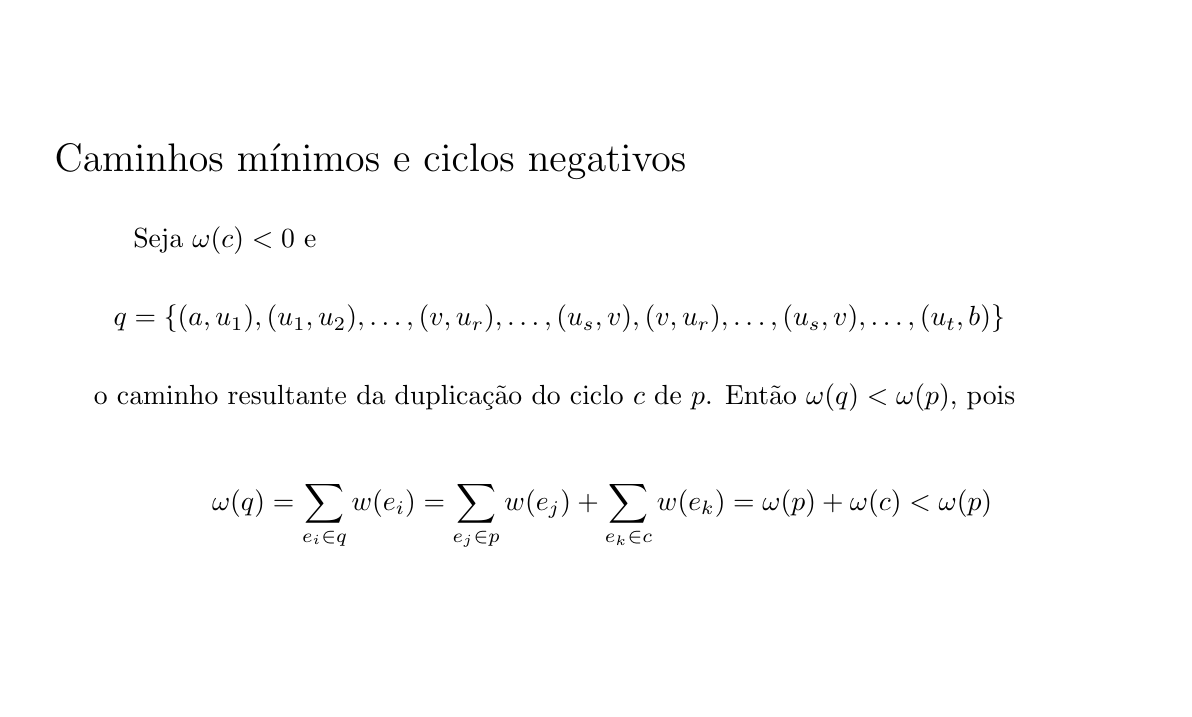
\begin{tikzpicture}
\node[draw,opacity=0] at (0, 0) {x};
\node[draw,opacity=0] at (14, 8) {x};
 \node[anchor=west] at (0, 6.5) { \Large \bbbold{Caminhos mínimos e ciclos negativos} };
 \node[anchor=west] at (1, 5.5) { \bbtext{Seja $\omega(c) < 0$ e } };
 \node[anchor=west] at (0.75, 4.5) { $q = \{ (a, u_1), (u_1, u_2), \ldots, (v, u_r), \dots, (u_s, v), (v, u_r), \ldots, (u_s, v), \ldots, (u_t, b) \}$ };
 \node[anchor=west] at (0.5, 3.5) { \bbtext{o caminho resultante da duplicação do ciclo $c$ de $p$. Então $\omega(q) < \omega(p)$, pois} };
 \node[anchor=west] at (2, 2) { $ \omega(q) = \displaystyle{\sum_{e_i\in q} w(e_i) = \sum_{e_j\in p} w(e_j) + \sum_{e_k\in c} w(e_k) = \omega(p) + \omega(c) < \omega(p)} $ };
\end{tikzpicture}
\end{frame}

\begin{frame}[plain,t]
\begin{tikzpicture}
\node[draw,opacity=0] at (0, 0) {x};
\node[draw,opacity=0] at (14, 8) {x};
 \node[circle, draw, very thick] (A) at (0.5, 7) { \bbtext{A} };
 \node[circle, draw, very thick] (B) at (6.5, 7) { \bbtext{B} };
 \node[circle, draw, very thick] (C) at (12.5, 7) { \bbtext{C} };
 \node[circle, draw, very thick] (D) at (9.5, 5) { \bbtext{D} };
 \node[circle, draw, very thick] (E) at (6.5, 3) { \bbtext{E} };
 \node[circle, draw, very thick] (F) at (3.5, 5) { \bbtext{F} };
 \draw[thick] (A) to node[below] { \bbinfo{1} } (B);
 \draw[thick] (B) to node[below] { \bbinfo{2} } (C);
 \draw[thick] (B) to node[below] { \bbinfo{3} } (D);
 \draw[thick] (D) to node[below] { \bbinfo{-4} } (E);
 \draw[thick] (E) to node[below] { \bbinfo{5} } (F);
 \draw[thick] (F) to node[below] { \bbinfo{-6} } (B);
\end{tikzpicture}
\end{frame}

\begin{frame}[plain,t]
\begin{tikzpicture}
\node[draw,opacity=0] at (0, 0) {x};
\node[draw,opacity=0] at (14, 8) {x};
 \node[circle, draw, very thick] (A) at (0.5, 7) { \bbtext{A} };
 \node[circle, draw, very thick] (B) at (6.5, 7) { \bbtext{B} };
 \node[circle, draw, very thick] (C) at (12.5, 7) { \bbtext{C} };
 \node[circle, draw, very thick] (D) at (9.5, 5) { \bbtext{D} };
 \node[circle, draw, very thick] (E) at (6.5, 3) { \bbtext{E} };
 \node[circle, draw, very thick] (F) at (3.5, 5) { \bbtext{F} };
 \draw[thick] (A) to node[below] { \bbinfo{1} } (B);
 \draw[thick] (B) to node[below] { \bbinfo{2} } (C);
 \draw[thick] (B) to node[below] { \bbinfo{3} } (D);
 \draw[thick] (D) to node[below] { \bbinfo{-4} } (E);
 \draw[thick] (E) to node[below] { \bbinfo{5} } (F);
 \draw[thick] (F) to node[below] { \bbinfo{-6} } (B);
 \draw[-latex,color=BBCyan] (1, 2) to (2, 2);
 \node[anchor=west] at (2, 2) { $p$ };
\end{tikzpicture}
\end{frame}

\begin{frame}[plain,t]
\begin{tikzpicture}
\node[draw,opacity=0] at (0, 0) {x};
\node[draw,opacity=0] at (14, 8) {x};
 \node[circle, draw, very thick] (A) at (0.5, 7) { \bbtext{A} };
 \node[circle, draw, very thick] (B) at (6.5, 7) { \bbtext{B} };
 \node[circle, draw, very thick] (C) at (12.5, 7) { \bbtext{C} };
 \node[circle, draw, very thick] (D) at (9.5, 5) { \bbtext{D} };
 \node[circle, draw, very thick] (E) at (6.5, 3) { \bbtext{E} };
 \node[circle, draw, very thick] (F) at (3.5, 5) { \bbtext{F} };
 \draw[thick] (B) to node[below] { \bbinfo{2} } (C);
 \draw[thick] (B) to node[below] { \bbinfo{3} } (D);
 \draw[thick] (D) to node[below] { \bbinfo{-4} } (E);
 \draw[thick] (E) to node[below] { \bbinfo{5} } (F);
 \draw[thick] (F) to node[below] { \bbinfo{-6} } (B);
 \draw[-latex,color=BBCyan] (1, 2) to (2, 2);
 \node[anchor=west] at (2, 2) { $p$ };
 \draw[-latex,very thick,color=BBCyan] (A) to node[below] { \bbinfo{1} } (B);
\end{tikzpicture}
\end{frame}

\begin{frame}[plain,t]
\begin{tikzpicture}
\node[draw,opacity=0] at (0, 0) {x};
\node[draw,opacity=0] at (14, 8) {x};
 \node[circle, draw, very thick] (A) at (0.5, 7) { \bbtext{A} };
 \node[circle, draw, very thick] (B) at (6.5, 7) { \bbtext{B} };
 \node[circle, draw, very thick] (C) at (12.5, 7) { \bbtext{C} };
 \node[circle, draw, very thick] (D) at (9.5, 5) { \bbtext{D} };
 \node[circle, draw, very thick] (E) at (6.5, 3) { \bbtext{E} };
 \node[circle, draw, very thick] (F) at (3.5, 5) { \bbtext{F} };
 \draw[thick] (B) to node[below] { \bbinfo{2} } (C);
 \draw[thick] (D) to node[below] { \bbinfo{-4} } (E);
 \draw[thick] (E) to node[below] { \bbinfo{5} } (F);
 \draw[thick] (F) to node[below] { \bbinfo{-6} } (B);
 \draw[-latex,color=BBCyan] (1, 2) to (2, 2);
 \node[anchor=west] at (2, 2) { $p$ };
 \draw[-latex,very thick,color=BBCyan] (A) to node[below] { \bbinfo{1} } (B);
 \draw[-latex,very thick,color=BBCyan] (B) to node[below] { \bbinfo{3} } (D);
\end{tikzpicture}
\end{frame}

\begin{frame}[plain,t]
\begin{tikzpicture}
\node[draw,opacity=0] at (0, 0) {x};
\node[draw,opacity=0] at (14, 8) {x};
 \node[circle, draw, very thick] (A) at (0.5, 7) { \bbtext{A} };
 \node[circle, draw, very thick] (B) at (6.5, 7) { \bbtext{B} };
 \node[circle, draw, very thick] (C) at (12.5, 7) { \bbtext{C} };
 \node[circle, draw, very thick] (D) at (9.5, 5) { \bbtext{D} };
 \node[circle, draw, very thick] (E) at (6.5, 3) { \bbtext{E} };
 \node[circle, draw, very thick] (F) at (3.5, 5) { \bbtext{F} };
 \draw[thick] (B) to node[below] { \bbinfo{2} } (C);
 \draw[thick] (E) to node[below] { \bbinfo{5} } (F);
 \draw[thick] (F) to node[below] { \bbinfo{-6} } (B);
 \draw[-latex,color=BBCyan] (1, 2) to (2, 2);
 \node[anchor=west] at (2, 2) { $p$ };
 \draw[-latex,very thick,color=BBCyan] (A) to node[below] { \bbinfo{1} } (B);
 \draw[-latex,very thick,color=BBCyan] (B) to node[below] { \bbinfo{3} } (D);
 \draw[-latex,very thick,color=BBCyan] (D) to node[below] { \bbinfo{-4} } (E);
\end{tikzpicture}
\end{frame}

\begin{frame}[plain,t]
\begin{tikzpicture}
\node[draw,opacity=0] at (0, 0) {x};
\node[draw,opacity=0] at (14, 8) {x};
 \node[circle, draw, very thick] (A) at (0.5, 7) { \bbtext{A} };
 \node[circle, draw, very thick] (B) at (6.5, 7) { \bbtext{B} };
 \node[circle, draw, very thick] (C) at (12.5, 7) { \bbtext{C} };
 \node[circle, draw, very thick] (D) at (9.5, 5) { \bbtext{D} };
 \node[circle, draw, very thick] (E) at (6.5, 3) { \bbtext{E} };
 \node[circle, draw, very thick] (F) at (3.5, 5) { \bbtext{F} };
 \draw[thick] (B) to node[below] { \bbinfo{2} } (C);
 \draw[thick] (F) to node[below] { \bbinfo{-6} } (B);
 \draw[-latex,color=BBCyan] (1, 2) to (2, 2);
 \node[anchor=west] at (2, 2) { $p$ };
 \draw[-latex,very thick,color=BBCyan] (A) to node[below] { \bbinfo{1} } (B);
 \draw[-latex,very thick,color=BBCyan] (B) to node[below] { \bbinfo{3} } (D);
 \draw[-latex,very thick,color=BBCyan] (D) to node[below] { \bbinfo{-4} } (E);
 \draw[-latex,very thick,color=BBCyan] (E) to node[below] { \bbinfo{5} } (F);
\end{tikzpicture}
\end{frame}

\begin{frame}[plain,t]
\begin{tikzpicture}
\node[draw,opacity=0] at (0, 0) {x};
\node[draw,opacity=0] at (14, 8) {x};
 \node[circle, draw, very thick] (A) at (0.5, 7) { \bbtext{A} };
 \node[circle, draw, very thick] (B) at (6.5, 7) { \bbtext{B} };
 \node[circle, draw, very thick] (C) at (12.5, 7) { \bbtext{C} };
 \node[circle, draw, very thick] (D) at (9.5, 5) { \bbtext{D} };
 \node[circle, draw, very thick] (E) at (6.5, 3) { \bbtext{E} };
 \node[circle, draw, very thick] (F) at (3.5, 5) { \bbtext{F} };
 \draw[thick] (B) to node[below] { \bbinfo{2} } (C);
 \draw[-latex,color=BBCyan] (1, 2) to (2, 2);
 \node[anchor=west] at (2, 2) { $p$ };
 \draw[-latex,very thick,color=BBCyan] (A) to node[below] { \bbinfo{1} } (B);
 \draw[-latex,very thick,color=BBCyan] (B) to node[below] { \bbinfo{3} } (D);
 \draw[-latex,very thick,color=BBCyan] (D) to node[below] { \bbinfo{-4} } (E);
 \draw[-latex,very thick,color=BBCyan] (E) to node[below] { \bbinfo{5} } (F);
 \draw[-latex,very thick,color=BBCyan] (F) to node[below] { \bbinfo{-6} } (B);
\end{tikzpicture}
\end{frame}

\begin{frame}[plain,t]
\begin{tikzpicture}
\node[draw,opacity=0] at (0, 0) {x};
\node[draw,opacity=0] at (14, 8) {x};
 \node[circle, draw, very thick] (A) at (0.5, 7) { \bbtext{A} };
 \node[circle, draw, very thick] (B) at (6.5, 7) { \bbtext{B} };
 \node[circle, draw, very thick] (C) at (12.5, 7) { \bbtext{C} };
 \node[circle, draw, very thick] (D) at (9.5, 5) { \bbtext{D} };
 \node[circle, draw, very thick] (E) at (6.5, 3) { \bbtext{E} };
 \node[circle, draw, very thick] (F) at (3.5, 5) { \bbtext{F} };
 \draw[-latex,color=BBCyan] (1, 2) to (2, 2);
 \node[anchor=west] at (2, 2) { $p$ };
 \draw[-latex,very thick,color=BBCyan] (A) to node[below] { \bbinfo{1} } (B);
 \draw[-latex,very thick,color=BBCyan] (B) to node[below] { \bbinfo{3} } (D);
 \draw[-latex,very thick,color=BBCyan] (D) to node[below] { \bbinfo{-4} } (E);
 \draw[-latex,very thick,color=BBCyan] (E) to node[below] { \bbinfo{5} } (F);
 \draw[-latex,very thick,color=BBCyan] (F) to node[below] { \bbinfo{-6} } (B);
 \draw[-latex,very thick,color=BBCyan] (B) to node[below] { \bbinfo{2} } (C);
\end{tikzpicture}
\end{frame}

\begin{frame}[plain,t]
\begin{tikzpicture}
\node[draw,opacity=0] at (0, 0) {x};
\node[draw,opacity=0] at (14, 8) {x};
 \node[circle, draw, very thick] (A) at (0.5, 7) { \bbtext{A} };
 \node[circle, draw, very thick] (B) at (6.5, 7) { \bbtext{B} };
 \node[circle, draw, very thick] (C) at (12.5, 7) { \bbtext{C} };
 \node[circle, draw, very thick] (D) at (9.5, 5) { \bbtext{D} };
 \node[circle, draw, very thick] (E) at (6.5, 3) { \bbtext{E} };
 \node[circle, draw, very thick] (F) at (3.5, 5) { \bbtext{F} };
 \draw[-latex,color=BBCyan] (1, 2) to (2, 2);
 \node[anchor=west] at (2, 2) { $p$ };
 \draw[-latex,very thick,color=BBCyan] (A) to node[below] { \bbinfo{1} } (B);
 \draw[-latex,very thick,color=BBCyan] (B) to node[below] { \bbinfo{3} } (D);
 \draw[-latex,very thick,color=BBCyan] (D) to node[below] { \bbinfo{-4} } (E);
 \draw[-latex,very thick,color=BBCyan] (E) to node[below] { \bbinfo{5} } (F);
 \draw[-latex,very thick,color=BBCyan] (F) to node[below] { \bbinfo{-6} } (B);
 \draw[-latex,very thick,color=BBCyan] (B) to node[below] { \bbinfo{2} } (C);
 \node[anchor=west] at (3, 2) { $\omega(p) = 3$ };
\end{tikzpicture}
\end{frame}

\begin{frame}[plain,t]
\begin{tikzpicture}
\node[draw,opacity=0] at (0, 0) {x};
\node[draw,opacity=0] at (14, 8) {x};
 \node[circle, draw, very thick] (A) at (0.5, 7) { \bbtext{A} };
 \node[circle, draw, very thick] (B) at (6.5, 7) { \bbtext{B} };
 \node[circle, draw, very thick] (C) at (12.5, 7) { \bbtext{C} };
 \node[circle, draw, very thick] (D) at (9.5, 5) { \bbtext{D} };
 \node[circle, draw, very thick] (E) at (6.5, 3) { \bbtext{E} };
 \node[circle, draw, very thick] (F) at (3.5, 5) { \bbtext{F} };
 \draw[-latex,color=BBCyan] (1, 2) to (2, 2);
 \node[anchor=west] at (2, 2) { $p$ };
 \node[anchor=west] at (3, 2) { $\omega(p) = 3$ };
 \draw[thick] (A) to node[below] { \bbinfo{1} } (B);
 \draw[thick] (B) to node[below] { \bbinfo{2} } (C);
 \draw[thick] (B) to node[below] { \bbinfo{3} } (D);
 \draw[thick] (D) to node[below] { \bbinfo{-4} } (E);
 \draw[thick] (E) to node[below] { \bbinfo{5} } (F);
 \draw[thick] (F) to node[below] { \bbinfo{-6} } (B);
 \draw[dashed,-latex,color=BBGreen] (1, 1) to (2, 1);
 \node[anchor=west] at (2, 1) { $q$ };
\end{tikzpicture}
\end{frame}

\begin{frame}[plain,t]
\begin{tikzpicture}
\node[draw,opacity=0] at (0, 0) {x};
\node[draw,opacity=0] at (14, 8) {x};
 \node[circle, draw, very thick] (A) at (0.5, 7) { \bbtext{A} };
 \node[circle, draw, very thick] (B) at (6.5, 7) { \bbtext{B} };
 \node[circle, draw, very thick] (C) at (12.5, 7) { \bbtext{C} };
 \node[circle, draw, very thick] (D) at (9.5, 5) { \bbtext{D} };
 \node[circle, draw, very thick] (E) at (6.5, 3) { \bbtext{E} };
 \node[circle, draw, very thick] (F) at (3.5, 5) { \bbtext{F} };
 \draw[-latex,color=BBCyan] (1, 2) to (2, 2);
 \node[anchor=west] at (2, 2) { $p$ };
 \node[anchor=west] at (3, 2) { $\omega(p) = 3$ };
 \draw[thick] (B) to node[below] { \bbinfo{2} } (C);
 \draw[thick] (B) to node[below] { \bbinfo{3} } (D);
 \draw[thick] (D) to node[below] { \bbinfo{-4} } (E);
 \draw[thick] (E) to node[below] { \bbinfo{5} } (F);
 \draw[thick] (F) to node[below] { \bbinfo{-6} } (B);
 \draw[dashed,-latex,color=BBGreen] (1, 1) to (2, 1);
 \node[anchor=west] at (2, 1) { $q$ };
 \draw[dashed,-latex,very thick,color=BBGreen] (A) to node[below] { \bbinfo{1} } (B);
\end{tikzpicture}
\end{frame}

\begin{frame}[plain,t]
\begin{tikzpicture}
\node[draw,opacity=0] at (0, 0) {x};
\node[draw,opacity=0] at (14, 8) {x};
 \node[circle, draw, very thick] (A) at (0.5, 7) { \bbtext{A} };
 \node[circle, draw, very thick] (B) at (6.5, 7) { \bbtext{B} };
 \node[circle, draw, very thick] (C) at (12.5, 7) { \bbtext{C} };
 \node[circle, draw, very thick] (D) at (9.5, 5) { \bbtext{D} };
 \node[circle, draw, very thick] (E) at (6.5, 3) { \bbtext{E} };
 \node[circle, draw, very thick] (F) at (3.5, 5) { \bbtext{F} };
 \draw[-latex,color=BBCyan] (1, 2) to (2, 2);
 \node[anchor=west] at (2, 2) { $p$ };
 \node[anchor=west] at (3, 2) { $\omega(p) = 3$ };
 \draw[thick] (B) to node[below] { \bbinfo{2} } (C);
 \draw[thick] (D) to node[below] { \bbinfo{-4} } (E);
 \draw[thick] (E) to node[below] { \bbinfo{5} } (F);
 \draw[thick] (F) to node[below] { \bbinfo{-6} } (B);
 \draw[dashed,-latex,color=BBGreen] (1, 1) to (2, 1);
 \node[anchor=west] at (2, 1) { $q$ };
 \draw[dashed,-latex,very thick,color=BBGreen] (A) to node[below] { \bbinfo{1} } (B);
 \draw[dashed,-latex,very thick,color=BBGreen] (B) to node[below] { \bbinfo{3} } (D);
\end{tikzpicture}
\end{frame}

\begin{frame}[plain,t]
\begin{tikzpicture}
\node[draw,opacity=0] at (0, 0) {x};
\node[draw,opacity=0] at (14, 8) {x};
 \node[circle, draw, very thick] (A) at (0.5, 7) { \bbtext{A} };
 \node[circle, draw, very thick] (B) at (6.5, 7) { \bbtext{B} };
 \node[circle, draw, very thick] (C) at (12.5, 7) { \bbtext{C} };
 \node[circle, draw, very thick] (D) at (9.5, 5) { \bbtext{D} };
 \node[circle, draw, very thick] (E) at (6.5, 3) { \bbtext{E} };
 \node[circle, draw, very thick] (F) at (3.5, 5) { \bbtext{F} };
 \draw[-latex,color=BBCyan] (1, 2) to (2, 2);
 \node[anchor=west] at (2, 2) { $p$ };
 \node[anchor=west] at (3, 2) { $\omega(p) = 3$ };
 \draw[thick] (B) to node[below] { \bbinfo{2} } (C);
 \draw[thick] (E) to node[below] { \bbinfo{5} } (F);
 \draw[thick] (F) to node[below] { \bbinfo{-6} } (B);
 \draw[dashed,-latex,color=BBGreen] (1, 1) to (2, 1);
 \node[anchor=west] at (2, 1) { $q$ };
 \draw[dashed,-latex,very thick,color=BBGreen] (A) to node[below] { \bbinfo{1} } (B);
 \draw[dashed,-latex,very thick,color=BBGreen] (B) to node[below] { \bbinfo{3} } (D);
 \draw[dashed,-latex,very thick,color=BBGreen] (D) to node[below] { \bbinfo{-4} } (E);
\end{tikzpicture}
\end{frame}

\begin{frame}[plain,t]
\begin{tikzpicture}
\node[draw,opacity=0] at (0, 0) {x};
\node[draw,opacity=0] at (14, 8) {x};
 \node[circle, draw, very thick] (A) at (0.5, 7) { \bbtext{A} };
 \node[circle, draw, very thick] (B) at (6.5, 7) { \bbtext{B} };
 \node[circle, draw, very thick] (C) at (12.5, 7) { \bbtext{C} };
 \node[circle, draw, very thick] (D) at (9.5, 5) { \bbtext{D} };
 \node[circle, draw, very thick] (E) at (6.5, 3) { \bbtext{E} };
 \node[circle, draw, very thick] (F) at (3.5, 5) { \bbtext{F} };
 \draw[-latex,color=BBCyan] (1, 2) to (2, 2);
 \node[anchor=west] at (2, 2) { $p$ };
 \node[anchor=west] at (3, 2) { $\omega(p) = 3$ };
 \draw[thick] (B) to node[below] { \bbinfo{2} } (C);
 \draw[thick] (F) to node[below] { \bbinfo{-6} } (B);
 \draw[dashed,-latex,color=BBGreen] (1, 1) to (2, 1);
 \node[anchor=west] at (2, 1) { $q$ };
 \draw[dashed,-latex,very thick,color=BBGreen] (A) to node[below] { \bbinfo{1} } (B);
 \draw[dashed,-latex,very thick,color=BBGreen] (B) to node[below] { \bbinfo{3} } (D);
 \draw[dashed,-latex,very thick,color=BBGreen] (D) to node[below] { \bbinfo{-4} } (E);
 \draw[dashed,-latex,very thick,color=BBGreen] (E) to node[below] { \bbinfo{5} } (F);
\end{tikzpicture}
\end{frame}

\begin{frame}[plain,t]
\begin{tikzpicture}
\node[draw,opacity=0] at (0, 0) {x};
\node[draw,opacity=0] at (14, 8) {x};
 \node[circle, draw, very thick] (A) at (0.5, 7) { \bbtext{A} };
 \node[circle, draw, very thick] (B) at (6.5, 7) { \bbtext{B} };
 \node[circle, draw, very thick] (C) at (12.5, 7) { \bbtext{C} };
 \node[circle, draw, very thick] (D) at (9.5, 5) { \bbtext{D} };
 \node[circle, draw, very thick] (E) at (6.5, 3) { \bbtext{E} };
 \node[circle, draw, very thick] (F) at (3.5, 5) { \bbtext{F} };
 \draw[-latex,color=BBCyan] (1, 2) to (2, 2);
 \node[anchor=west] at (2, 2) { $p$ };
 \node[anchor=west] at (3, 2) { $\omega(p) = 3$ };
 \draw[thick] (B) to node[below] { \bbinfo{2} } (C);
 \draw[dashed,-latex,color=BBGreen] (1, 1) to (2, 1);
 \node[anchor=west] at (2, 1) { $q$ };
 \draw[dashed,-latex,very thick,color=BBGreen] (A) to node[below] { \bbinfo{1} } (B);
 \draw[dashed,-latex,very thick,color=BBGreen] (B) to node[below] { \bbinfo{3} } (D);
 \draw[dashed,-latex,very thick,color=BBGreen] (D) to node[below] { \bbinfo{-4} } (E);
 \draw[dashed,-latex,very thick,color=BBGreen] (E) to node[below] { \bbinfo{5} } (F);
 \draw[dashed,-latex,very thick,color=BBGreen] (F) to node[below] { \bbinfo{-6} } (B);
\end{tikzpicture}
\end{frame}

\begin{frame}[plain,t]
\begin{tikzpicture}
\node[draw,opacity=0] at (0, 0) {x};
\node[draw,opacity=0] at (14, 8) {x};
 \node[circle, draw, very thick] (A) at (0.5, 7) { \bbtext{A} };
 \node[circle, draw, very thick] (B) at (6.5, 7) { \bbtext{B} };
 \node[circle, draw, very thick] (C) at (12.5, 7) { \bbtext{C} };
 \node[circle, draw, very thick] (D) at (9.5, 5) { \bbtext{D} };
 \node[circle, draw, very thick] (E) at (6.5, 3) { \bbtext{E} };
 \node[circle, draw, very thick] (F) at (3.5, 5) { \bbtext{F} };
 \draw[-latex,color=BBCyan] (1, 2) to (2, 2);
 \node[anchor=west] at (2, 2) { $p$ };
 \node[anchor=west] at (3, 2) { $\omega(p) = 3$ };
 \draw[thick] (B) to node[below] { \bbinfo{2} } (C);
 \draw[dashed,-latex,color=BBGreen] (1, 1) to (2, 1);
 \node[anchor=west] at (2, 1) { $q$ };
 \draw[dashed,-latex,very thick,color=BBGreen] (A) to node[below] { \bbinfo{1} } (B);
 \draw[dashed,-latex,very thick,color=BBGreen] (B) to node[below] { \bbinfo{3} } (D);
 \draw[dashed,-latex,very thick,color=BBGreen] (D) to node[below] { \bbinfo{-4} } (E);
 \draw[dashed,-latex,very thick,color=BBGreen] (E) to node[below] { \bbinfo{5} } (F);
 \draw[dashed,-latex,very thick,color=BBGreen] (F) to node[below] { \bbinfo{-6} } (B);
 \draw[very thick,-latex,color=BBGreen,dashed] (B) to [bend left] (D);
\end{tikzpicture}
\end{frame}

\begin{frame}[plain,t]
\begin{tikzpicture}
\node[draw,opacity=0] at (0, 0) {x};
\node[draw,opacity=0] at (14, 8) {x};
 \node[circle, draw, very thick] (A) at (0.5, 7) { \bbtext{A} };
 \node[circle, draw, very thick] (B) at (6.5, 7) { \bbtext{B} };
 \node[circle, draw, very thick] (C) at (12.5, 7) { \bbtext{C} };
 \node[circle, draw, very thick] (D) at (9.5, 5) { \bbtext{D} };
 \node[circle, draw, very thick] (E) at (6.5, 3) { \bbtext{E} };
 \node[circle, draw, very thick] (F) at (3.5, 5) { \bbtext{F} };
 \draw[-latex,color=BBCyan] (1, 2) to (2, 2);
 \node[anchor=west] at (2, 2) { $p$ };
 \node[anchor=west] at (3, 2) { $\omega(p) = 3$ };
 \draw[thick] (B) to node[below] { \bbinfo{2} } (C);
 \draw[dashed,-latex,color=BBGreen] (1, 1) to (2, 1);
 \node[anchor=west] at (2, 1) { $q$ };
 \draw[dashed,-latex,very thick,color=BBGreen] (A) to node[below] { \bbinfo{1} } (B);
 \draw[dashed,-latex,very thick,color=BBGreen] (B) to node[below] { \bbinfo{3} } (D);
 \draw[dashed,-latex,very thick,color=BBGreen] (D) to node[below] { \bbinfo{-4} } (E);
 \draw[dashed,-latex,very thick,color=BBGreen] (E) to node[below] { \bbinfo{5} } (F);
 \draw[dashed,-latex,very thick,color=BBGreen] (F) to node[below] { \bbinfo{-6} } (B);
 \draw[very thick,-latex,color=BBGreen,dashed] (B) to [bend left] (D);
 \draw[very thick,-latex,color=BBGreen,dashed] (D) to [bend left] (E);
\end{tikzpicture}
\end{frame}

\begin{frame}[plain,t]
\begin{tikzpicture}
\node[draw,opacity=0] at (0, 0) {x};
\node[draw,opacity=0] at (14, 8) {x};
 \node[circle, draw, very thick] (A) at (0.5, 7) { \bbtext{A} };
 \node[circle, draw, very thick] (B) at (6.5, 7) { \bbtext{B} };
 \node[circle, draw, very thick] (C) at (12.5, 7) { \bbtext{C} };
 \node[circle, draw, very thick] (D) at (9.5, 5) { \bbtext{D} };
 \node[circle, draw, very thick] (E) at (6.5, 3) { \bbtext{E} };
 \node[circle, draw, very thick] (F) at (3.5, 5) { \bbtext{F} };
 \draw[-latex,color=BBCyan] (1, 2) to (2, 2);
 \node[anchor=west] at (2, 2) { $p$ };
 \node[anchor=west] at (3, 2) { $\omega(p) = 3$ };
 \draw[thick] (B) to node[below] { \bbinfo{2} } (C);
 \draw[dashed,-latex,color=BBGreen] (1, 1) to (2, 1);
 \node[anchor=west] at (2, 1) { $q$ };
 \draw[dashed,-latex,very thick,color=BBGreen] (A) to node[below] { \bbinfo{1} } (B);
 \draw[dashed,-latex,very thick,color=BBGreen] (B) to node[below] { \bbinfo{3} } (D);
 \draw[dashed,-latex,very thick,color=BBGreen] (D) to node[below] { \bbinfo{-4} } (E);
 \draw[dashed,-latex,very thick,color=BBGreen] (E) to node[below] { \bbinfo{5} } (F);
 \draw[dashed,-latex,very thick,color=BBGreen] (F) to node[below] { \bbinfo{-6} } (B);
 \draw[very thick,-latex,color=BBGreen,dashed] (B) to [bend left] (D);
 \draw[very thick,-latex,color=BBGreen,dashed] (D) to [bend left] (E);
 \draw[very thick,-latex,color=BBGreen,dashed] (E) to [bend left] (F);
\end{tikzpicture}
\end{frame}

\begin{frame}[plain,t]
\begin{tikzpicture}
\node[draw,opacity=0] at (0, 0) {x};
\node[draw,opacity=0] at (14, 8) {x};
 \node[circle, draw, very thick] (A) at (0.5, 7) { \bbtext{A} };
 \node[circle, draw, very thick] (B) at (6.5, 7) { \bbtext{B} };
 \node[circle, draw, very thick] (C) at (12.5, 7) { \bbtext{C} };
 \node[circle, draw, very thick] (D) at (9.5, 5) { \bbtext{D} };
 \node[circle, draw, very thick] (E) at (6.5, 3) { \bbtext{E} };
 \node[circle, draw, very thick] (F) at (3.5, 5) { \bbtext{F} };
 \draw[-latex,color=BBCyan] (1, 2) to (2, 2);
 \node[anchor=west] at (2, 2) { $p$ };
 \node[anchor=west] at (3, 2) { $\omega(p) = 3$ };
 \draw[thick] (B) to node[below] { \bbinfo{2} } (C);
 \draw[dashed,-latex,color=BBGreen] (1, 1) to (2, 1);
 \node[anchor=west] at (2, 1) { $q$ };
 \draw[dashed,-latex,very thick,color=BBGreen] (A) to node[below] { \bbinfo{1} } (B);
 \draw[dashed,-latex,very thick,color=BBGreen] (B) to node[below] { \bbinfo{3} } (D);
 \draw[dashed,-latex,very thick,color=BBGreen] (D) to node[below] { \bbinfo{-4} } (E);
 \draw[dashed,-latex,very thick,color=BBGreen] (E) to node[below] { \bbinfo{5} } (F);
 \draw[dashed,-latex,very thick,color=BBGreen] (F) to node[below] { \bbinfo{-6} } (B);
 \draw[very thick,-latex,color=BBGreen,dashed] (B) to [bend left] (D);
 \draw[very thick,-latex,color=BBGreen,dashed] (D) to [bend left] (E);
 \draw[very thick,-latex,color=BBGreen,dashed] (E) to [bend left] (F);
 \draw[very thick,-latex,color=BBGreen,dashed] (F) to [bend left] (B);
\end{tikzpicture}
\end{frame}

\begin{frame}[plain,t]
\begin{tikzpicture}
\node[draw,opacity=0] at (0, 0) {x};
\node[draw,opacity=0] at (14, 8) {x};
 \node[circle, draw, very thick] (A) at (0.5, 7) { \bbtext{A} };
 \node[circle, draw, very thick] (B) at (6.5, 7) { \bbtext{B} };
 \node[circle, draw, very thick] (C) at (12.5, 7) { \bbtext{C} };
 \node[circle, draw, very thick] (D) at (9.5, 5) { \bbtext{D} };
 \node[circle, draw, very thick] (E) at (6.5, 3) { \bbtext{E} };
 \node[circle, draw, very thick] (F) at (3.5, 5) { \bbtext{F} };
 \draw[-latex,color=BBCyan] (1, 2) to (2, 2);
 \node[anchor=west] at (2, 2) { $p$ };
 \node[anchor=west] at (3, 2) { $\omega(p) = 3$ };
 \draw[dashed,-latex,color=BBGreen] (1, 1) to (2, 1);
 \node[anchor=west] at (2, 1) { $q$ };
 \draw[dashed,-latex,very thick,color=BBGreen] (A) to node[below] { \bbinfo{1} } (B);
 \draw[dashed,-latex,very thick,color=BBGreen] (B) to node[below] { \bbinfo{3} } (D);
 \draw[dashed,-latex,very thick,color=BBGreen] (D) to node[below] { \bbinfo{-4} } (E);
 \draw[dashed,-latex,very thick,color=BBGreen] (E) to node[below] { \bbinfo{5} } (F);
 \draw[dashed,-latex,very thick,color=BBGreen] (F) to node[below] { \bbinfo{-6} } (B);
 \draw[very thick,-latex,color=BBGreen,dashed] (B) to [bend left] (D);
 \draw[very thick,-latex,color=BBGreen,dashed] (D) to [bend left] (E);
 \draw[very thick,-latex,color=BBGreen,dashed] (E) to [bend left] (F);
 \draw[very thick,-latex,color=BBGreen,dashed] (F) to [bend left] (B);
 \draw[dashed,-latex,very thick,color=BBGreen] (B) to node[below] { \bbinfo{2} } (C);
\end{tikzpicture}
\end{frame}

\begin{frame}[plain,t]
\begin{tikzpicture}
\node[draw,opacity=0] at (0, 0) {x};
\node[draw,opacity=0] at (14, 8) {x};
 \node[circle, draw, very thick] (A) at (0.5, 7) { \bbtext{A} };
 \node[circle, draw, very thick] (B) at (6.5, 7) { \bbtext{B} };
 \node[circle, draw, very thick] (C) at (12.5, 7) { \bbtext{C} };
 \node[circle, draw, very thick] (D) at (9.5, 5) { \bbtext{D} };
 \node[circle, draw, very thick] (E) at (6.5, 3) { \bbtext{E} };
 \node[circle, draw, very thick] (F) at (3.5, 5) { \bbtext{F} };
 \draw[-latex,color=BBCyan] (1, 2) to (2, 2);
 \node[anchor=west] at (2, 2) { $p$ };
 \node[anchor=west] at (3, 2) { $\omega(p) = 3$ };
 \draw[dashed,-latex,color=BBGreen] (1, 1) to (2, 1);
 \node[anchor=west] at (2, 1) { $q$ };
 \draw[dashed,-latex,very thick,color=BBGreen] (A) to node[below] { \bbinfo{1} } (B);
 \draw[dashed,-latex,very thick,color=BBGreen] (B) to node[below] { \bbinfo{3} } (D);
 \draw[dashed,-latex,very thick,color=BBGreen] (D) to node[below] { \bbinfo{-4} } (E);
 \draw[dashed,-latex,very thick,color=BBGreen] (E) to node[below] { \bbinfo{5} } (F);
 \draw[dashed,-latex,very thick,color=BBGreen] (F) to node[below] { \bbinfo{-6} } (B);
 \draw[very thick,-latex,color=BBGreen,dashed] (B) to [bend left] (D);
 \draw[very thick,-latex,color=BBGreen,dashed] (D) to [bend left] (E);
 \draw[very thick,-latex,color=BBGreen,dashed] (E) to [bend left] (F);
 \draw[very thick,-latex,color=BBGreen,dashed] (F) to [bend left] (B);
 \draw[dashed,-latex,very thick,color=BBGreen] (B) to node[below] { \bbinfo{2} } (C);
 \node[anchor=west] at (3, 1) { $\omega(q) = 1$ };
\end{tikzpicture}
\end{frame}

\begin{frame}[plain,t]
\begin{tikzpicture}
\node[draw,opacity=0] at (0, 0) {x};
\node[draw,opacity=0] at (14, 8) {x};
 \node[anchor=west] at (0, 6.5) { \Large \bbbold{Número de rodadas do algoritmo de Bellman-Ford} };
\end{tikzpicture}
\end{frame}

\begin{frame}[plain,t]
\begin{tikzpicture}
\node[draw,opacity=0] at (0, 0) {x};
\node[draw,opacity=0] at (14, 8) {x};
 \node[anchor=west] at (0, 6.5) { \Large \bbbold{Número de rodadas do algoritmo de Bellman-Ford} };
 \node[anchor=west] at (1, 5) { \bbtext{\bbbold{Teorema.} Seja $G(V, E)$ um grafo cujos pesos de suas arestas sejam todos } };
 \node[anchor=west] at (0.5, 4) { \bbtext{não-negativos. Então para qualquer $v\in V$, o caminho mínimo de $s$ a $u$ iden-} };
 \node[anchor=west] at (0.5, 3) { \bbtext{tificado pelo algoritmo de Bellman-Ford tem, no máximo, $|V| - 1$ arestas. } };
\end{tikzpicture}
\end{frame}

\begin{frame}[plain,t]
\begin{tikzpicture}
\node[draw,opacity=0] at (0, 0) {x};
\node[draw,opacity=0] at (14, 8) {x};
 \node[anchor=west] at (0, 6.5) { \Large \bbbold{Detecção de ciclos negativos} };
\end{tikzpicture}
\end{frame}

\begin{frame}[plain,t]
\begin{tikzpicture}
\node[draw,opacity=0] at (0, 0) {x};
\node[draw,opacity=0] at (14, 8) {x};
 \node[anchor=west] at (0, 6.5) { \Large \bbbold{Detecção de ciclos negativos} };
 \node[anchor=west] at (1, 5) { \bbtext{\bbbold{Teorema.} Seja $G(V, E)$ um grafo. Se a $|V|$-ésima rodada do algoritmo de } };
 \node[anchor=west] at (0.5, 4) { \bbtext{Bellman-Ford atualizar o vetor $d$ ao menos uma vez, então $G$ possui pelo menos } };
 \node[anchor=west] at (0.5, 3) { \bbtext{um ciclo negativo. } };
\end{tikzpicture}
\end{frame}

\begin{frame}[plain,t]
 \begin{center}\inputsnippet{cpp}{6}{22}{codes/negative-cycle.cpp}\end{center}
\end{frame}

\begin{frame}[plain,t]
\begin{tikzpicture}
\node[draw,opacity=0] at (0, 0) {x};
\node[draw,opacity=0] at (14, 8) {x};
 \node[anchor=west] at (0, 6) { \Large \bbbold{Problemas sugeridos} };
 \node[anchor=west] at (1, 5) { $1.$ \bbtext{AtCoder Beginner Contest 088 -- Problem D: Repainting } };
 \node[anchor=west] at (1, 4) { $2.$ \bbtext{Codeforces Beta Round \#3 -- Problem A: Shortest path of the king } };
 \node[anchor=west] at (1, 3) { $3.$ \bbtext{OJ 10000 -- Longest Paths } };
 \node[anchor=west] at (1, 2) { $4.$ \bbtext{OJ 10959 -- The Party, Part I } };
\end{tikzpicture}
\end{frame}

\begin{frame}[plain,t]
\begin{tikzpicture}
\node[draw,opacity=0] at (0, 0) {x};
\node[draw,opacity=0] at (14, 8) {x};
 \node[anchor=west] at (0, 7) { \Large \bbbold{Referências} };
 \node[anchor=west] at (1, 6) { $1.$ \bbbold{HALIM}, \bbtext{Felix}; \bbbold{HALIM}, \bbtext{Steve}. \bbenglish{Competitive Programming 3,} \bbtext{2010.} };
 \node[anchor=west] at (1, 5) { $2.$ \bbbold{LAAKSONEN}, \bbtext{Antti}. \bbenglish{Competitive Programmer's Handbook,} \bbtext{2018.} };
 \node[anchor=west] at (1, 4) { $3.$ \bbbold{SKIENA}, \bbtext{Steven}; \bbbold{REVILLA}, \bbtext{Miguel}. \bbenglish{Programming Challenges,} \bbtext{2003.} };
 \node[anchor=west] at (1, 3) { $4.$ \bbbold{Wikipédia}, \bbenglish{Bellman-Ford algorithm.} \bbtext{Acesso em 07/07/2021.} };
 \node[anchor=west] at (1, 2) { $5.$ \bbbold{Wikipédia}, \bbenglish{L. R. Ford Jr.} \bbtext{Acesso em 07/07/2021.} };
 \node[anchor=west] at (1, 1) { $6.$ \bbbold{Wikipédia}, \bbenglish{Richard E. Bellman.} \bbtext{Acesso em 07/07/2021.} };
\end{tikzpicture}
\end{frame}

\end{document}
